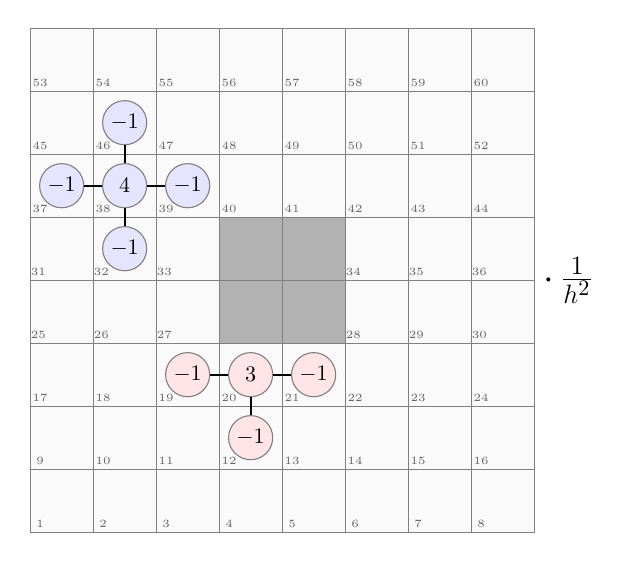
\begin{tikzpicture}
[
 scale=0.8,
 every node/.style ={scale=0.8},
 inner sep=0.5mm,
 BLUECIRC/.style={circle, draw=black!50, fill=blue!10,  thin, minimum size=7.0mm},
 REDCIRC/.style={circle, draw=black!50, fill=red!10, thin, minimum size=7.0mm},
 OBST/.style={rectangle, draw=black!50, fill=black!30, thin, minimum size=10mm},
 CELL/.style={rectangle, draw=black!50, fill=black!02,   thin, minimum size=10mm},
 ],
%      
\foreach \y in {1,2,3,4,5,6,7,8}
   \foreach \x in {1,2,3,4,5,6,7,8}
      {
        \node [CELL]    at ( \x, \y)  {};
       }
\foreach \y in {4,5}
   \foreach \x in {4,5} { \node [OBST]    at ( \x, \y)  {}; }
%
\node  at (9.0,4.5)  {\LARGE \,$\cdot \,\frac{1}{h^2}$};       
%
\node [REDCIRC]  (XS)   at ( 4, 2)  {$-1$};
\node [REDCIRC]  (XW)   at ( 3, 3)  {$-1$};
\node [REDCIRC]  (XC)   at ( 4, 3)  {$3$};
\node [REDCIRC]  (XE)   at ( 5, 3)  {$-1$};
%
\node [BLUECIRC]  (YS)   at ( 2, 5)  {$-1$};
\node [BLUECIRC]  (YW)   at ( 1, 6)  {$-1$};
\node [BLUECIRC]  (YC)   at ( 2, 6)  {$4$};
\node [BLUECIRC]  (YN)   at ( 2, 7)  {$-1$};
\node [BLUECIRC]  (YE)   at ( 3, 6)  {$-1$};
%
\draw [thick]  (XC.south) -- (XS.north) ;
\draw [thick]  (XC.west)  -- (XW.east) ;
\draw [thick]  (XC.east)  -- (XE.west) ;
%
\draw [thick]  (YC.south) -- (YS.north) ;
\draw [thick]  (YC.west)  -- (YW.east) ;
\draw [thick]  (YC.east)  -- (YE.west) ;
\draw [thick]  (YC.north) -- (YN.south) ;
%
\pgfmathsetmacro{\num}{int(0)}
\foreach \y in {0,1,2} {
  \pgfmathsetmacro{\ypos}{(\y+0.63)}
  \foreach \x in {0,1,2,3,4,5,6,7} {
    \pgfmathsetmacro{\xpos}{(\x+0.66)}
    \pgfmathsetmacro{\num}{int(8*\y+\x+1)}
    \draw[color=black!60]   node at (\xpos,\ypos) {\tiny \num};
  }
}
%
\draw[color=black!60]   node at (0.63,3.63) {\tiny 25};
\draw[color=black!60]   node at (1.63,3.63) {\tiny 26};
\draw[color=black!60]   node at (2.63,3.63) {\tiny 27};
\draw[color=black!60]   node at (5.63,3.63) {\tiny 28};
\draw[color=black!60]   node at (6.63,3.63) {\tiny 29};
\draw[color=black!60]   node at (7.63,3.63) {\tiny 30};
%
\draw[color=black!60]   node at (0.63,4.63) {\tiny 31};
\draw[color=black!60]   node at (1.63,4.63) {\tiny 32};
\draw[color=black!60]   node at (2.63,4.63) {\tiny 33};
\draw[color=black!60]   node at (5.63,4.63) {\tiny 34};
\draw[color=black!60]   node at (6.63,4.63) {\tiny 35};
\draw[color=black!60]   node at (7.63,4.63) {\tiny 36};
%
\foreach \y in {5,6,7} {
  \pgfmathsetmacro{\ypos}{(\y+0.63)}
  \foreach \x in {0,1,2,3,4,5,6,7} {
    \pgfmathsetmacro{\xpos}{(\x+0.66)}
    \pgfmathsetmacro{\num}{int(8*\y+\x-3)}
    \draw[color=black!60]   node at (\xpos,\ypos) {\tiny \num};
  }
}
%
\end{tikzpicture}
